\section{Entwurfsphase}

\subsection{Architekturdesign}
\label{Architekturdesign}

Als passendes Entwurfsmuster für den Shortcut Editor hat sich das Model View Presenter (MVP)-Architekturmuster herausgestellt. Dieses ist nicht ganz so verbreitet wie das bekanntere Model View Controller (MVC)-Muster, ist diesem aber sehr ähnlich. Der eigendliche Unterschied zwischen MVP und MVC liegt darin, dass bei MVC die View neben dem Controller auch mit dem Model kommuniziert und dieses somit kennen muss. Bei MVP ist die View völlig unabhängig vom Model und nur der Presenter kommuniziert mit ihr (siehe \autoref{fig:modelview}). Der Autor hat sich für das MVP-Entwurfsmuster entschieden, da damit die View auch ohne Model verwendet werden kann und es denkbar ist, das diese Möglichkeit in Zukunft benötigt wird.

\begin{figure}[H] 
	\subfloat{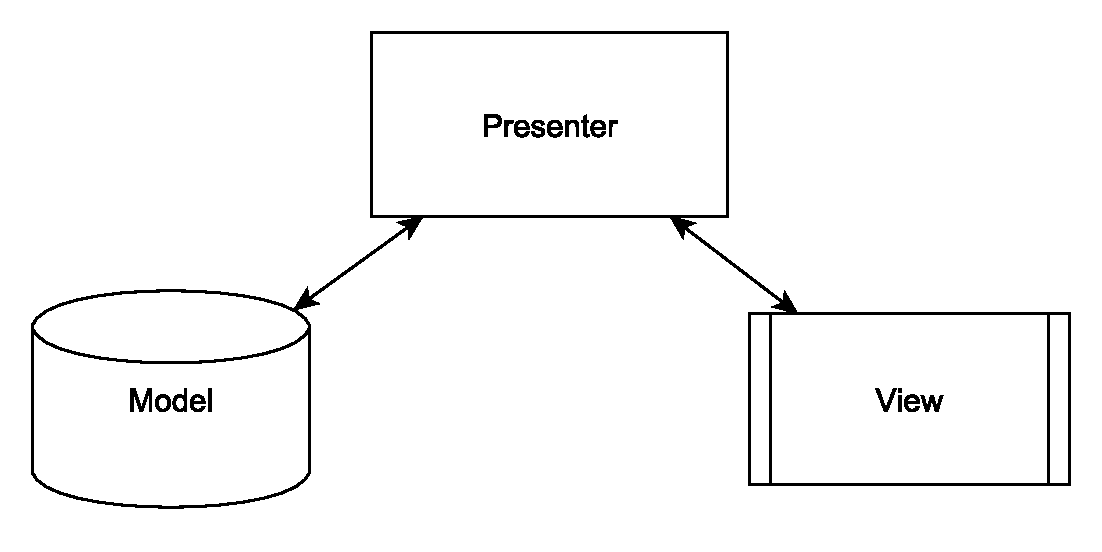
\includegraphics[width=0.5\textwidth-5px]{../graphic/diagrams/ModelViewPresenter/ModelViewPresenter}}
	\hfill 
	\subfloat{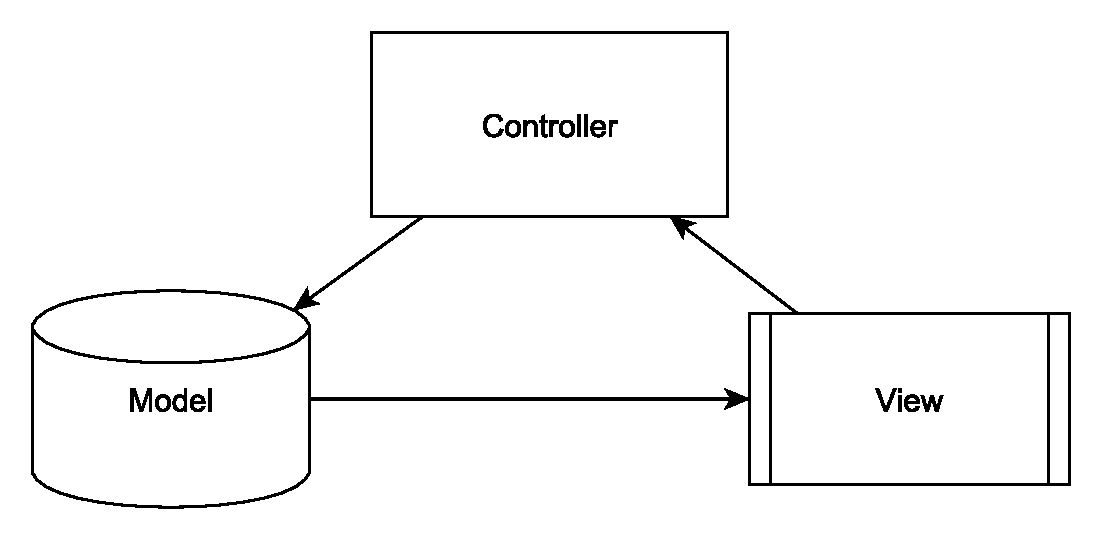
\includegraphics[width=0.5\textwidth-5px]{../graphic/diagrams/ModelViewController/ModelViewController}}
	\caption{Model View Presenter vs. Model View Controller} 
	\label{fig:modelview}
\end{figure}

Bei MVP lässt sich jede Komponente der Software einem der drei Bestandteile - Model, View oder Presenter - zuordnen. Jeder dieser Teile hat einen eigenen Aufgabenbereich, der von denen der anderen weitestgehend unabhängig ist. Im Model werden alle Daten gehalten und zur Verfügung gestellt. Die View kümmert sich um die grafische Darstellung und der Presenter stellt das Bindeglied zwischen der View und dem Model dar. Verändern sich beispielsweiße die Werte in der View, so kümmert sich der Presenter darum, dass diese Wertänderung im Model ebenso stattfindet und andersherum. Der Presenter hält somit die View -- oder auch mehrere Views untereinander -- und das Model auf dem gleichen stand. Die lose Kopplung der einzelnen Komponenten erhöht die Wiederverwendbarkeit und Austauschbarkeit. Man könnte beispielsweise die Benutzeroberfläche austauschen, ohne das Model anpassen zu müssen. Außerdem können die einzelnen Komponenten durch die strikte Trennung einfacher getestet, gewartet und flexibel erweitert werden. Diese Vorteile sprechen ebenso für eine Verwendung von MVP.

\vfill

Im Sinne der Wiederverwendbarkeit, werden auch alle GUI-Komponenten des Shortcut Editors völlig seperat voneinander und unabhängig vom Editor implementiert. Dadurch kann gewährleistet werden, keine unnötigen Abhängigkeiten zu editorspezifischen Teilen aufzubauen. So ist die Benutzung von Komponenten auch an anderen Stellen in der Software ohne weiteren Aufwand möglich.

\vfill

Wie im Abschnitt \ref{schnittstellen} bereits erwähnt, wird für das Lesen der Testergebnis XML-Dateien das hauseigene Propertly Framework verwendet. Dieses Tool stellt Funktionalitäten zum Lesen und Schreiben von XML zur Verfügung. Außerdem kümmert es sich eigendständig um die Konvertierung von Datentypen. Dadurch kommt der Autor bei der Implementierung nicht mit XML spezifischen Arbeiten in Berührung und kann sich auf den eigentlichen Editor konzentrieren.

\newpage

\subsection{Benutzeroberfläche}
\label{ui}

Für das Design des User Interfaces (UI) wurden von einem UX-Designer der ADITO Software GmbH Entwürfe angefertigt (siehe \autoref{fig:uxDesigns}). Im Designentwurf wird ersichtlich, welche Komponenten verwendet werden müssen, um alle angeforderten Informationen darzustellen und wie diese aussehen und angeordet zu sein haben, um die bedarfsgerechte Bedienung zu ermöglichen. Nachfolgend werden die Bestandteile des Editors näher erläutert:

\ding{192} \textbf{Breadcrumb:} Diese Komponente ist in der Lage einen Pfad darzustellen und diesen zu bearbeiten. In diesem Fall besteht sie aus beliebig vielen ComboBoxen, um an jeder Stelle des Pfads einen anderen Knoten auswählen zu können. Diese Komponente dient zum Einen als Orientierungshilfe, um jederzeit feststellen zu können, für welche Aktion der Shortcut gesetzt wird. Zum Anderen ist damit eine intuitive Navigation durch alle Aktionen möglich.

\ding{193} \textbf{Shortcut-Field:} Hierbei handelt es sich um eine Komponente, welche die Darstellung und Bearbeitung von Shortcuts ermöglicht. Die Eingabe und Editierung des Tastaturkürzels kann nur bei fokusiertem Zustand erfolgen. Demnach wechselt die Komponente bei Fokusierung in den Bearbeitungsmodus und verlässt diesen, sobald eine andere Komponente den Fokus erlangt.

\ding{194} \textbf{Check-Button:} Dieses GUI-Element kann selektiert werden und stellt neben einem Icon ein Häckchen- oder Kreuzsymbol dar. Somit kann die Komponente visualisieren, bei welchem Browser bzw. Betriebssystem der Shortcut Probleme bereiten kann (Kreuz) und wo dieser unbedenklich ist (Häckchen). Außerdem dient sie dem Benutzer zur Auswahl eines Elements, um davon mehr Informationen zu erhalten (Im Entwurf werden beispielhaft für Google Chrome und macOS detailierte Informationen angezeigt).

\ding{195} \textbf{Shortcut-Tag:} Ein Shortcut-Tag dient zur Darstellung einer Tastenkombination und bietet die Möglichkeit sich mittles eines Kreuz-Buttons selber zu entfernen.

\ding{196} \textbf{TreeTable:} Zur Darstellung der zugrundeliegenden Baumstruktur wird zur Visualisierung aller Aktionen eine Kombination aus Tree und Tabelle verwendet. Sie dient -- wie die \textbf{Breadcrumb} -- der Navigation und bietet zudem einen Überblick über alle vorhandenen Shortcuts.

\ding{197} \textbf{Accordion:} Ist ein \textbf{Check-Button} selektiert, so wird eine Accordion-Komponente angezeigt, welche detailierte Informationen zu den Testergebnissen bietet. Um nur relevante Daten anzuzeigen, besteht die Möglichkeit einige Sektionen durch Klicken auf den Header einzuklappen.

\begin{figure}[H] 
	\begin{overpic}[width=1\linewidth,unit=1px]%
		{../graphic/images/ux/Kombination}
		\put(75,175){\ding{182}}
		\put(134,163){\ding{183}}
		\put(217,149){\ding{184}}
		\put(34,149){\ding{184}}
		\put(375,80){\ding{184}}
		
		\put(185,110){\ding{185}}
		\put(185,101){\ding{185}}
		
		\put(185,82){\ding{185}}
		\put(185,73){\ding{185}}
		
		\put(185,56){\ding{185}}
		
		\put(185,37){\ding{185}}
		\put(185,27){\ding{185}}
		
		\put(110,79){\ding{186}}
		\put(280,137){\ding{187}}
		\put(280,68){\ding{187}}
		
	\end{overpic}

	\caption{Designentwurf des UX-Designers}
	\label{fig:uxDesigns}
\end{figure}

\newpage

\subsection{Datenmodell für Entitäten und Aktionen}
\label{DatenmodellFunc}

\begin{wrapfigure}[17]{r}[0cm]{200px}
	\vspace{-12px}
	\centering
	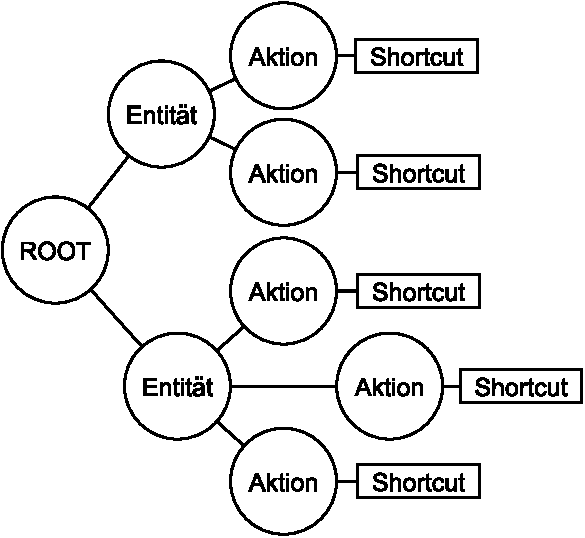
\includegraphics[width=200px]{../graphic/diagrams/Baumstruktur_Functions/Baumstruktur}
	\caption{Baumstruktur für Entitäten und Funktionen}
	\label{fig:baumstruktur_Func}
\end{wrapfigure}

Wie sich im Designentwurf (\autoref{fig:uxDesigns}) -- aufgrund der TreeTable -- schon erahnen lässt, sollen die Entitäten und deren Aktionen als Baumstruktur aufgebaut werden. Jede Aktion stellt einen Endknoten (Blatt) dar und soll genau einen Shortcut besitzen können. Entitäten hingegen ist es nur erlaubt, Aktionen und weitere Entitäten aufzunehmen (siehe \autoref{fig:baumstruktur_Func}). Da es sich um eine Baumstruktur handelt, kann man ausschließen, dass sich eine Entität selbst als Kind hält.

Um diese Struktur im Editor abbilden zu können, wurde ein Datenmodell entworfen, welches den Anforderungen entspricht. Zur Erläuterung des Models ist im Folgenden ein schematisches UML Klassendiagramm abgebildet, welches den Grundaufbau und die Beziehungen zwischen den Elementen verdeutlicht (\autoref{fig:baumstrukturUML_Func}).

\vfill

Zentraler Bestandteil des Datenmodells ist das Interface \textbf{IEditorShortcutNode}. Dieses kann neben einem eigenen Namen auch seine Kinder zurückgeben. Diese sind ebenfalls vom Typ \textbf{IEditorShortcutNode}. Damit kann grundsätzlich schon eine Baumstrukturen aufgebaut werden. Allerdings ist durch \textbf{IEditorShortcutNode} nur die Abbildung der Bestandteile \textbf{ROOT} und \textbf{Entity} aus \autoref{fig:baumstruktur_Func} möglich, da noch kein Tastenkürzel gehalten werden kann.

\vfill

\begin{figure}[H]
	\vspace{20px}
	\centering
	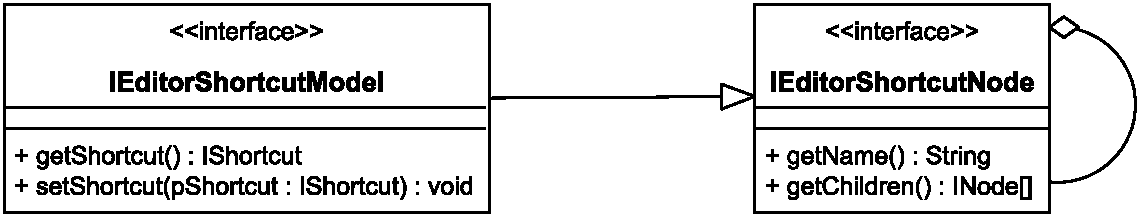
\includegraphics[height=57px]{../graphic/diagrams/CD_Baumstruktur_Functions/Baumstruktur}
	\caption{Datenmodell für Entitäten und Aktionen}
	\label{fig:baumstrukturUML_Func}
\end{figure}

\vfill

Um auch eine Aktion im Modell abbilden zu können, existiert das Interface \textbf{IEditorShortcutModel}. Dieses erbt von \textbf{IEditorShortcutNode} und stellt somit einen vollwertigen Knoten dar, welcher bei der Methode \textbf{getChildren()} zurückgegeben werden kann. Über die Methoden \textbf{setShortcut(...)} kann eine Tastenkombination gesetzt und über \textbf{getShortcut()} ausgelesen werden. Da diese Methoden nur die Zuweisung von einem einzigen Shortcut zulassen, ist sichergestellt, dass eine Aktion nur ein Tastenkürzel besitzen kann. Aufgrund der Tatsache, dass \textbf{IEditorShortcutModel} einen Endknoten (Blatt) darstellt und somit keine Kinder hat, liefert die geerbte Methode \textbf{getChildren()} ein leeres Array. Für die Iteration durch den Baum ist es programmatisch konfortabler und effizienter, wenn jeder Knoten die Methode \textbf{getChildren()} besitzt, da andernfalls unnötige Abfragen stattfinden müssen.

Über diese Konstellation lässt sich die Baumstruktur der Aktionen und deren Shortcuts den Anforderungen entsprechend abbilden.

\newpage

\subsection{Datenmodell für Browsertestergebnisse}
\label{DatenmodellBrow}

\begin{wrapfigure}[9]{l}[0cm]{165px}
	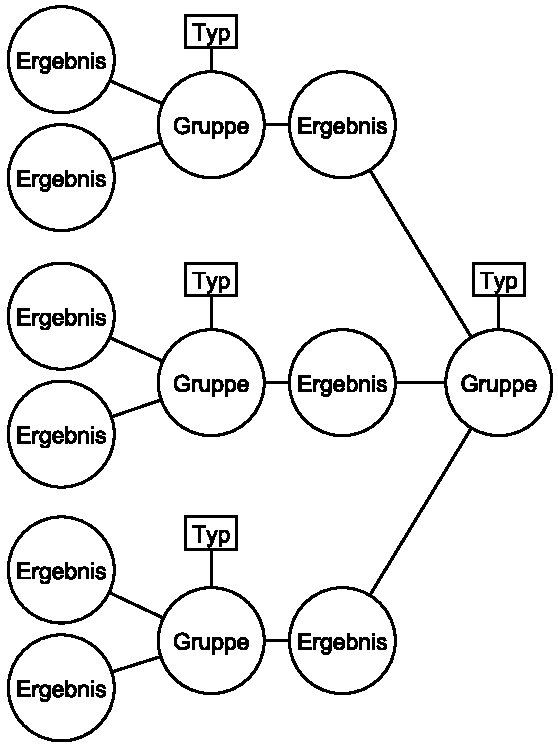
\includegraphics[width=165px]{../graphic/diagrams/Baumstruktur_Results/Baumstruktur}
	\caption{Baumstruktur für Browsertestergebnisse}
	\label{fig:baumstruktur_Result}
\end{wrapfigure}

Auch die Browserergebnisse werden als Baumstruktur gehalten. Allerdings ergiebt sich hierbei eine neue Anforderung. Betrachtet man den Designentwurf, so stellt man fest, dass eine Gruppe von Testergebnissen immer eine Typenbezeichnung hat (Im Entwurf haben die Gruppen den Typ \glqq Browser\grqq\xspace oder \glqq Betriebssystem\grqq). In \autoref{fig:baumstrukturUML_Results} ist ein UML-Klassendiagramm eines Datenmodells abgebildet, welches den Anforderungen zum Halten von Browsertestergebnissen gerecht wird.

\begin{figure}[H]
	\flushright
	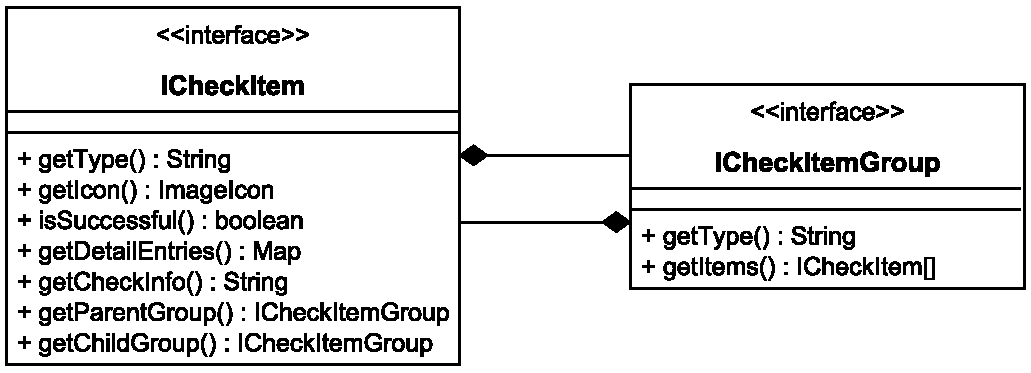
\includegraphics[width=280px]{../graphic/diagrams/CD_Baumstruktur_Results/Baumstruktur}
	\captionsetup{width=235px, justification=raggedleft}
	\caption{Datenmodell für Browsertestergebnisse}
	\label{fig:baumstrukturUML_Results}
\end{figure}

In diesem Modell stellt ein \textbf{ICheckItem} ein einzelnes Testergbnis dar. Eine \textbf{ICheckItemGroup} hält neben einer beliebigen Anzahl von \textbf{ICheckItem}s einen Typ in Form eines \textbf{String}s. Somit kann zu jeder Gruppe die gewünschte Typenbezeichnung hinzugefügt werden. Ein \textbf{ICheckItem} besitzt eine Parent- und ein Childgruppe. Diese können mittels der Methoden \textbf{getParentGroup} und \textbf{getChildGroup} erlangt werden. Über diese Methoden lässt sich durch die Baumstruktur iterieren.

\vspace{-5px}

\subsection{Datenstore}

Damit sowohl die Daten der Entitäten und Aktionen als auch die der Browsertestergebnissen in zuvor geschilderter Form erhalten werden können, soll ein Datenstore zum Einsatz kommen. Dieser liefert die beiden oben beschriebenen Datenmodelle. Dabei kümmert er sich die Daten von anderen Quellen (z.B. XML-Dateien) in die gewünschte Datenmodell-Form zu bringen. Zudem ist er dafür zuständig, die geänderten Daten wieder zurück zu speichern.

Um auch ohne die Integration des ShortcutEditors in den ADTIO Designer testweise Entitäten und deren Aktionen zur Verfügung zu haben, soll ein DummyStore implementiert werden, welcher fiktive Testdaten in die Datenmodelle einfügt.

\vfill

\begin{figure}[H]
	\centering
	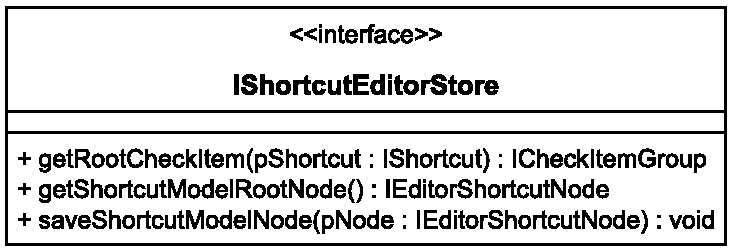
\includegraphics[height=70px]{../graphic/diagrams/CD_IShortcutEditorStore/IShortcutEditorStore}
	\caption{Datenstore}
	\label{fig:ishortcuteditorstore}
\end{figure}



\newpage